% generated by make_figs.py from a real FastBandSolver run; do not edit by hand
\begin{figure}[p]
\centering
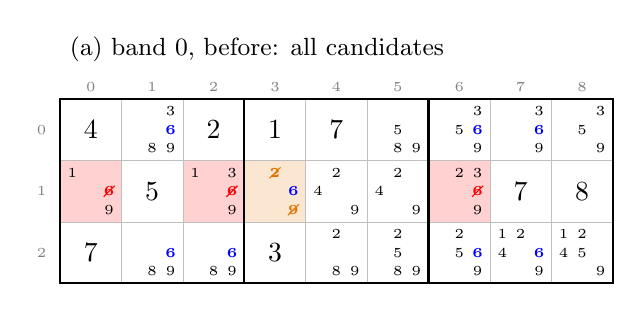
\begin{tikzpicture}[x=1cm,y=1cm]
\node[anchor=south west,font=\small] at (0,2.690) {(a) band 0, before: all candidates};
\node[font=\normalsize,text=black] at (0.390,1.950) {4};
\node[font=\tiny,text=black,inner sep=0] at (1.404,2.184) {3};
\node[font=\tiny\bfseries,text=blue,inner sep=0] at (1.404,1.950) {6};
\node[font=\tiny,text=black,inner sep=0] at (1.170,1.716) {8};
\node[font=\tiny,text=black,inner sep=0] at (1.404,1.716) {9};
\node[font=\normalsize,text=black] at (1.950,1.950) {2};
\node[font=\normalsize,text=black] at (2.730,1.950) {1};
\node[font=\normalsize,text=black] at (3.510,1.950) {7};
\node[font=\tiny,text=black,inner sep=0] at (4.290,1.950) {5};
\node[font=\tiny,text=black,inner sep=0] at (4.290,1.716) {8};
\node[font=\tiny,text=black,inner sep=0] at (4.524,1.716) {9};
\node[font=\tiny,text=black,inner sep=0] at (5.304,2.184) {3};
\node[font=\tiny,text=black,inner sep=0] at (5.070,1.950) {5};
\node[font=\tiny\bfseries,text=blue,inner sep=0] at (5.304,1.950) {6};
\node[font=\tiny,text=black,inner sep=0] at (5.304,1.716) {9};
\node[font=\tiny,text=black,inner sep=0] at (6.084,2.184) {3};
\node[font=\tiny\bfseries,text=blue,inner sep=0] at (6.084,1.950) {6};
\node[font=\tiny,text=black,inner sep=0] at (6.084,1.716) {9};
\node[font=\tiny,text=black,inner sep=0] at (6.864,2.184) {3};
\node[font=\tiny,text=black,inner sep=0] at (6.630,1.950) {5};
\node[font=\tiny,text=black,inner sep=0] at (6.864,1.716) {9};
\fill[red!18] (0.000,0.780) rectangle (0.780,1.560);
\node[font=\tiny,text=black,inner sep=0] at (0.156,1.404) {1};
\node[font=\tiny\bfseries,text=red,inner sep=0] at (0.624,1.170) {6};
\draw[red,thin] (0.554,1.100) -- (0.694,1.240);
\node[font=\tiny,text=black,inner sep=0] at (0.624,0.936) {9};
\node[font=\normalsize,text=black] at (1.170,1.170) {5};
\fill[red!18] (1.560,0.780) rectangle (2.340,1.560);
\node[font=\tiny,text=black,inner sep=0] at (1.716,1.404) {1};
\node[font=\tiny,text=black,inner sep=0] at (2.184,1.404) {3};
\node[font=\tiny\bfseries,text=red,inner sep=0] at (2.184,1.170) {6};
\draw[red,thin] (2.114,1.100) -- (2.254,1.240);
\node[font=\tiny,text=black,inner sep=0] at (2.184,0.936) {9};
\fill[orange!90!black!18] (2.340,0.780) rectangle (3.120,1.560);
\node[font=\tiny\bfseries,text=orange!90!black,inner sep=0] at (2.730,1.404) {2};
\draw[orange!90!black,thin] (2.660,1.334) -- (2.800,1.474);
\node[font=\tiny\bfseries,text=blue,inner sep=0] at (2.964,1.170) {6};
\node[font=\tiny\bfseries,text=orange!90!black,inner sep=0] at (2.964,0.936) {9};
\draw[orange!90!black,thin] (2.894,0.866) -- (3.034,1.006);
\node[font=\tiny,text=black,inner sep=0] at (3.510,1.404) {2};
\node[font=\tiny,text=black,inner sep=0] at (3.276,1.170) {4};
\node[font=\tiny,text=black,inner sep=0] at (3.744,0.936) {9};
\node[font=\tiny,text=black,inner sep=0] at (4.290,1.404) {2};
\node[font=\tiny,text=black,inner sep=0] at (4.056,1.170) {4};
\node[font=\tiny,text=black,inner sep=0] at (4.524,0.936) {9};
\fill[red!18] (4.680,0.780) rectangle (5.460,1.560);
\node[font=\tiny,text=black,inner sep=0] at (5.070,1.404) {2};
\node[font=\tiny,text=black,inner sep=0] at (5.304,1.404) {3};
\node[font=\tiny\bfseries,text=red,inner sep=0] at (5.304,1.170) {6};
\draw[red,thin] (5.234,1.100) -- (5.374,1.240);
\node[font=\tiny,text=black,inner sep=0] at (5.304,0.936) {9};
\node[font=\normalsize,text=black] at (5.850,1.170) {7};
\node[font=\normalsize,text=black] at (6.630,1.170) {8};
\node[font=\normalsize,text=black] at (0.390,0.390) {7};
\node[font=\tiny\bfseries,text=blue,inner sep=0] at (1.404,0.390) {6};
\node[font=\tiny,text=black,inner sep=0] at (1.170,0.156) {8};
\node[font=\tiny,text=black,inner sep=0] at (1.404,0.156) {9};
\node[font=\tiny\bfseries,text=blue,inner sep=0] at (2.184,0.390) {6};
\node[font=\tiny,text=black,inner sep=0] at (1.950,0.156) {8};
\node[font=\tiny,text=black,inner sep=0] at (2.184,0.156) {9};
\node[font=\normalsize,text=black] at (2.730,0.390) {3};
\node[font=\tiny,text=black,inner sep=0] at (3.510,0.624) {2};
\node[font=\tiny,text=black,inner sep=0] at (3.510,0.156) {8};
\node[font=\tiny,text=black,inner sep=0] at (3.744,0.156) {9};
\node[font=\tiny,text=black,inner sep=0] at (4.290,0.624) {2};
\node[font=\tiny,text=black,inner sep=0] at (4.290,0.390) {5};
\node[font=\tiny,text=black,inner sep=0] at (4.290,0.156) {8};
\node[font=\tiny,text=black,inner sep=0] at (4.524,0.156) {9};
\node[font=\tiny,text=black,inner sep=0] at (5.070,0.624) {2};
\node[font=\tiny,text=black,inner sep=0] at (5.070,0.390) {5};
\node[font=\tiny\bfseries,text=blue,inner sep=0] at (5.304,0.390) {6};
\node[font=\tiny,text=black,inner sep=0] at (5.304,0.156) {9};
\node[font=\tiny,text=black,inner sep=0] at (5.616,0.624) {1};
\node[font=\tiny,text=black,inner sep=0] at (5.850,0.624) {2};
\node[font=\tiny,text=black,inner sep=0] at (5.616,0.390) {4};
\node[font=\tiny\bfseries,text=blue,inner sep=0] at (6.084,0.390) {6};
\node[font=\tiny,text=black,inner sep=0] at (6.084,0.156) {9};
\node[font=\tiny,text=black,inner sep=0] at (6.396,0.624) {1};
\node[font=\tiny,text=black,inner sep=0] at (6.630,0.624) {2};
\node[font=\tiny,text=black,inner sep=0] at (6.396,0.390) {4};
\node[font=\tiny,text=black,inner sep=0] at (6.630,0.390) {5};
\node[font=\tiny,text=black,inner sep=0] at (6.864,0.156) {9};
\draw[step=0.78,gray!50,very thin] (0,0) grid (7.020,2.340);
\draw[thick] (2.340,0) -- (2.340,2.340);
\draw[thick] (4.680,0) -- (4.680,2.340);
\draw[thick] (0,0) rectangle (7.020,2.340);
\node[font=\tiny,text=gray] at (0.390,2.490) {0};
\node[font=\tiny,text=gray] at (1.170,2.490) {1};
\node[font=\tiny,text=gray] at (1.950,2.490) {2};
\node[font=\tiny,text=gray] at (2.730,2.490) {3};
\node[font=\tiny,text=gray] at (3.510,2.490) {4};
\node[font=\tiny,text=gray] at (4.290,2.490) {5};
\node[font=\tiny,text=gray] at (5.070,2.490) {6};
\node[font=\tiny,text=gray] at (5.850,2.490) {7};
\node[font=\tiny,text=gray] at (6.630,2.490) {8};
\node[font=\tiny,text=gray,anchor=east] at (-0.05,1.950) {0};
\node[font=\tiny,text=gray,anchor=east] at (-0.05,1.170) {1};
\node[font=\tiny,text=gray,anchor=east] at (-0.05,0.390) {2};
\end{tikzpicture}
\hspace{0.6cm}
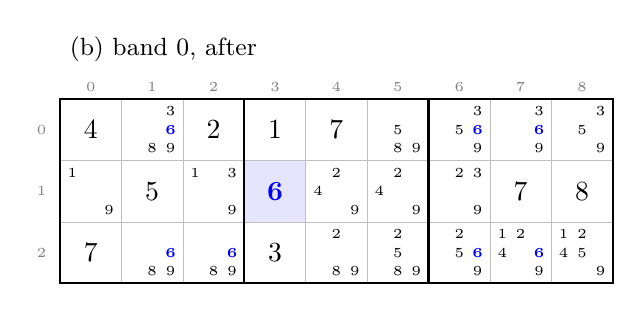
\begin{tikzpicture}[x=1cm,y=1cm]
\node[anchor=south west,font=\small] at (0,2.690) {(b) band 0, after};
\node[font=\normalsize,text=black] at (0.390,1.950) {4};
\node[font=\tiny,text=black,inner sep=0] at (1.404,2.184) {3};
\node[font=\tiny\bfseries,text=blue,inner sep=0] at (1.404,1.950) {6};
\node[font=\tiny,text=black,inner sep=0] at (1.170,1.716) {8};
\node[font=\tiny,text=black,inner sep=0] at (1.404,1.716) {9};
\node[font=\normalsize,text=black] at (1.950,1.950) {2};
\node[font=\normalsize,text=black] at (2.730,1.950) {1};
\node[font=\normalsize,text=black] at (3.510,1.950) {7};
\node[font=\tiny,text=black,inner sep=0] at (4.290,1.950) {5};
\node[font=\tiny,text=black,inner sep=0] at (4.290,1.716) {8};
\node[font=\tiny,text=black,inner sep=0] at (4.524,1.716) {9};
\node[font=\tiny,text=black,inner sep=0] at (5.304,2.184) {3};
\node[font=\tiny,text=black,inner sep=0] at (5.070,1.950) {5};
\node[font=\tiny\bfseries,text=blue,inner sep=0] at (5.304,1.950) {6};
\node[font=\tiny,text=black,inner sep=0] at (5.304,1.716) {9};
\node[font=\tiny,text=black,inner sep=0] at (6.084,2.184) {3};
\node[font=\tiny\bfseries,text=blue,inner sep=0] at (6.084,1.950) {6};
\node[font=\tiny,text=black,inner sep=0] at (6.084,1.716) {9};
\node[font=\tiny,text=black,inner sep=0] at (6.864,2.184) {3};
\node[font=\tiny,text=black,inner sep=0] at (6.630,1.950) {5};
\node[font=\tiny,text=black,inner sep=0] at (6.864,1.716) {9};
\node[font=\tiny,text=black,inner sep=0] at (0.156,1.404) {1};
\node[font=\tiny,text=black,inner sep=0] at (0.624,0.936) {9};
\node[font=\normalsize,text=black] at (1.170,1.170) {5};
\node[font=\tiny,text=black,inner sep=0] at (1.716,1.404) {1};
\node[font=\tiny,text=black,inner sep=0] at (2.184,1.404) {3};
\node[font=\tiny,text=black,inner sep=0] at (2.184,0.936) {9};
\fill[blue!10] (2.340,0.780) rectangle (3.120,1.560);
\node[font=\normalsize\bfseries,text=blue] at (2.730,1.170) {6};
\node[font=\tiny,text=black,inner sep=0] at (3.510,1.404) {2};
\node[font=\tiny,text=black,inner sep=0] at (3.276,1.170) {4};
\node[font=\tiny,text=black,inner sep=0] at (3.744,0.936) {9};
\node[font=\tiny,text=black,inner sep=0] at (4.290,1.404) {2};
\node[font=\tiny,text=black,inner sep=0] at (4.056,1.170) {4};
\node[font=\tiny,text=black,inner sep=0] at (4.524,0.936) {9};
\node[font=\tiny,text=black,inner sep=0] at (5.070,1.404) {2};
\node[font=\tiny,text=black,inner sep=0] at (5.304,1.404) {3};
\node[font=\tiny,text=black,inner sep=0] at (5.304,0.936) {9};
\node[font=\normalsize,text=black] at (5.850,1.170) {7};
\node[font=\normalsize,text=black] at (6.630,1.170) {8};
\node[font=\normalsize,text=black] at (0.390,0.390) {7};
\node[font=\tiny\bfseries,text=blue,inner sep=0] at (1.404,0.390) {6};
\node[font=\tiny,text=black,inner sep=0] at (1.170,0.156) {8};
\node[font=\tiny,text=black,inner sep=0] at (1.404,0.156) {9};
\node[font=\tiny\bfseries,text=blue,inner sep=0] at (2.184,0.390) {6};
\node[font=\tiny,text=black,inner sep=0] at (1.950,0.156) {8};
\node[font=\tiny,text=black,inner sep=0] at (2.184,0.156) {9};
\node[font=\normalsize,text=black] at (2.730,0.390) {3};
\node[font=\tiny,text=black,inner sep=0] at (3.510,0.624) {2};
\node[font=\tiny,text=black,inner sep=0] at (3.510,0.156) {8};
\node[font=\tiny,text=black,inner sep=0] at (3.744,0.156) {9};
\node[font=\tiny,text=black,inner sep=0] at (4.290,0.624) {2};
\node[font=\tiny,text=black,inner sep=0] at (4.290,0.390) {5};
\node[font=\tiny,text=black,inner sep=0] at (4.290,0.156) {8};
\node[font=\tiny,text=black,inner sep=0] at (4.524,0.156) {9};
\node[font=\tiny,text=black,inner sep=0] at (5.070,0.624) {2};
\node[font=\tiny,text=black,inner sep=0] at (5.070,0.390) {5};
\node[font=\tiny\bfseries,text=blue,inner sep=0] at (5.304,0.390) {6};
\node[font=\tiny,text=black,inner sep=0] at (5.304,0.156) {9};
\node[font=\tiny,text=black,inner sep=0] at (5.616,0.624) {1};
\node[font=\tiny,text=black,inner sep=0] at (5.850,0.624) {2};
\node[font=\tiny,text=black,inner sep=0] at (5.616,0.390) {4};
\node[font=\tiny\bfseries,text=blue,inner sep=0] at (6.084,0.390) {6};
\node[font=\tiny,text=black,inner sep=0] at (6.084,0.156) {9};
\node[font=\tiny,text=black,inner sep=0] at (6.396,0.624) {1};
\node[font=\tiny,text=black,inner sep=0] at (6.630,0.624) {2};
\node[font=\tiny,text=black,inner sep=0] at (6.396,0.390) {4};
\node[font=\tiny,text=black,inner sep=0] at (6.630,0.390) {5};
\node[font=\tiny,text=black,inner sep=0] at (6.864,0.156) {9};
\draw[step=0.78,gray!50,very thin] (0,0) grid (7.020,2.340);
\draw[thick] (2.340,0) -- (2.340,2.340);
\draw[thick] (4.680,0) -- (4.680,2.340);
\draw[thick] (0,0) rectangle (7.020,2.340);
\node[font=\tiny,text=gray] at (0.390,2.490) {0};
\node[font=\tiny,text=gray] at (1.170,2.490) {1};
\node[font=\tiny,text=gray] at (1.950,2.490) {2};
\node[font=\tiny,text=gray] at (2.730,2.490) {3};
\node[font=\tiny,text=gray] at (3.510,2.490) {4};
\node[font=\tiny,text=gray] at (4.290,2.490) {5};
\node[font=\tiny,text=gray] at (5.070,2.490) {6};
\node[font=\tiny,text=gray] at (5.850,2.490) {7};
\node[font=\tiny,text=gray] at (6.630,2.490) {8};
\node[font=\tiny,text=gray,anchor=east] at (-0.05,1.950) {0};
\node[font=\tiny,text=gray,anchor=east] at (-0.05,1.170) {1};
\node[font=\tiny,text=gray,anchor=east] at (-0.05,0.390) {2};
\end{tikzpicture}
\\[0.5cm]
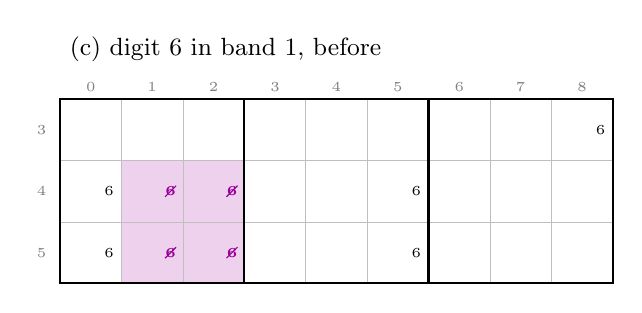
\begin{tikzpicture}[x=1cm,y=1cm]
\node[anchor=south west,font=\small] at (0,2.690) {(c) digit 6 in band 1, before};
\node[font=\tiny,text=black,inner sep=0] at (6.864,1.950) {6};
\node[font=\tiny,text=black,inner sep=0] at (0.624,1.170) {6};
\fill[violet!80!magenta!18] (0.780,0.780) rectangle (1.560,1.560);
\node[font=\tiny\bfseries,text=violet!80!magenta,inner sep=0] at (1.404,1.170) {6};
\draw[violet!80!magenta,thin] (1.334,1.100) -- (1.474,1.240);
\fill[violet!80!magenta!18] (1.560,0.780) rectangle (2.340,1.560);
\node[font=\tiny\bfseries,text=violet!80!magenta,inner sep=0] at (2.184,1.170) {6};
\draw[violet!80!magenta,thin] (2.114,1.100) -- (2.254,1.240);
\node[font=\tiny,text=black,inner sep=0] at (4.524,1.170) {6};
\node[font=\tiny,text=black,inner sep=0] at (0.624,0.390) {6};
\fill[violet!80!magenta!18] (0.780,0.000) rectangle (1.560,0.780);
\node[font=\tiny\bfseries,text=violet!80!magenta,inner sep=0] at (1.404,0.390) {6};
\draw[violet!80!magenta,thin] (1.334,0.320) -- (1.474,0.460);
\fill[violet!80!magenta!18] (1.560,0.000) rectangle (2.340,0.780);
\node[font=\tiny\bfseries,text=violet!80!magenta,inner sep=0] at (2.184,0.390) {6};
\draw[violet!80!magenta,thin] (2.114,0.320) -- (2.254,0.460);
\node[font=\tiny,text=black,inner sep=0] at (4.524,0.390) {6};
\draw[step=0.78,gray!50,very thin] (0,0) grid (7.020,2.340);
\draw[thick] (2.340,0) -- (2.340,2.340);
\draw[thick] (4.680,0) -- (4.680,2.340);
\draw[thick] (0,0) rectangle (7.020,2.340);
\node[font=\tiny,text=gray] at (0.390,2.490) {0};
\node[font=\tiny,text=gray] at (1.170,2.490) {1};
\node[font=\tiny,text=gray] at (1.950,2.490) {2};
\node[font=\tiny,text=gray] at (2.730,2.490) {3};
\node[font=\tiny,text=gray] at (3.510,2.490) {4};
\node[font=\tiny,text=gray] at (4.290,2.490) {5};
\node[font=\tiny,text=gray] at (5.070,2.490) {6};
\node[font=\tiny,text=gray] at (5.850,2.490) {7};
\node[font=\tiny,text=gray] at (6.630,2.490) {8};
\node[font=\tiny,text=gray,anchor=east] at (-0.05,1.950) {3};
\node[font=\tiny,text=gray,anchor=east] at (-0.05,1.170) {4};
\node[font=\tiny,text=gray,anchor=east] at (-0.05,0.390) {5};
\end{tikzpicture}
\hspace{0.6cm}
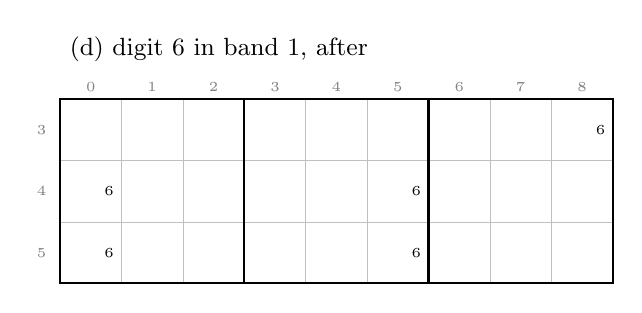
\begin{tikzpicture}[x=1cm,y=1cm]
\node[anchor=south west,font=\small] at (0,2.690) {(d) digit 6 in band 1, after};
\node[font=\tiny,text=black,inner sep=0] at (6.864,1.950) {6};
\node[font=\tiny,text=black,inner sep=0] at (0.624,1.170) {6};
\node[font=\tiny,text=black,inner sep=0] at (4.524,1.170) {6};
\node[font=\tiny,text=black,inner sep=0] at (0.624,0.390) {6};
\node[font=\tiny,text=black,inner sep=0] at (4.524,0.390) {6};
\draw[step=0.78,gray!50,very thin] (0,0) grid (7.020,2.340);
\draw[thick] (2.340,0) -- (2.340,2.340);
\draw[thick] (4.680,0) -- (4.680,2.340);
\draw[thick] (0,0) rectangle (7.020,2.340);
\node[font=\tiny,text=gray] at (0.390,2.490) {0};
\node[font=\tiny,text=gray] at (1.170,2.490) {1};
\node[font=\tiny,text=gray] at (1.950,2.490) {2};
\node[font=\tiny,text=gray] at (2.730,2.490) {3};
\node[font=\tiny,text=gray] at (3.510,2.490) {4};
\node[font=\tiny,text=gray] at (4.290,2.490) {5};
\node[font=\tiny,text=gray] at (5.070,2.490) {6};
\node[font=\tiny,text=gray] at (5.850,2.490) {7};
\node[font=\tiny,text=gray] at (6.630,2.490) {8};
\node[font=\tiny,text=gray,anchor=east] at (-0.05,1.950) {3};
\node[font=\tiny,text=gray,anchor=east] at (-0.05,1.170) {4};
\node[font=\tiny,text=gray,anchor=east] at (-0.05,0.390) {5};
\end{tikzpicture}
\\[0.5cm]
{\small (e) bookkeeping for digit 6, band 0\\[2pt]
\begin{tabular}{lll}\toprule field & before & after \\ \midrule
\texttt{cells}$[5\cdot 3+0]$ (digit 6, band 0) & \texttt{306\,115\,302}$_8$ & \texttt{306\,010\,302}$_8$ \\
\texttt{checked}$[5\cdot 3+0]$ & \texttt{347\,155\,342}$_8$ & \texttt{306\,010\,302}$_8$ \\
\texttt{openRows}$[5]$ (rows 8\ldots 0) & \texttt{110\,110\,111} & \texttt{110\,110\,101} \\
\texttt{unsolved}$[0]$ & \texttt{766\,175\,742}$_8$ & \texttt{766\,165\,742}$_8$ \\
\bottomrule\end{tabular}}
\caption{\textsc{UpdateBand} (\cref{alg:band}) on digit 6 in band 0, taken from a real run on magictour puzzle 96. Small digits are candidates, large digits are solved cells, and digit 6 is blue. Struck-out candidates are the ones this call removes, coloured by the step that removes them: \textcolor{red}{red} by the band rule (line 3), \textcolor{orange!90!black}{orange} by the row-single placement (lines 10--16), \textcolor{violet!80!magenta}{violet} by the stack rule (line 7); cells that lose a candidate are shaded in the same colour. The band rule removes 6 from row 1 at columns 0, 2, 6, which leaves column 3 as the only place for 6 in row 1; so the row-single step places it there, shaded blue in (b), and removes 2 and 9 from that cell. Because band 0's set of columns for 6 changed, the stack rule runs and removes 6 from 4 cells of band 1, (c) and (d); these are in band 1, so they appear only in (c). In (e), the mask shrinks, \texttt{checked} records the band-rule result, row 1 leaves \texttt{openRows}, and the placed cell leaves \texttt{unsolved} (its bit 12).}
\label{fig:alg-band}
\end{figure}
